% CENTRAL QUESTION:
% How does the elasticity of substitution between effective AI production services and human labor
% shape economic growth, wages, interest rates, and the functional distribution
% of income when frontier AI research is autonomous?
%
% BENCHMARK SCOPE:
% Autonomous AI research. The benchmark contains no H, omega_H, or sigma_HM.
% See REWRITE_AXM_PLAN.md before adding any result, equation, table, or figure.

\documentclass[11pt]{article}

\usepackage[margin=1in]{geometry}
\usepackage{amsmath,amssymb,amsthm,mathtools}
\usepackage{booktabs,array}
\usepackage{graphicx}
\usepackage{float}
\usepackage{tikz}
\usetikzlibrary{arrows.meta,positioning}
\usepackage{microtype}
\usepackage{setspace}
\usepackage{needspace}
\usepackage{enumitem}
\usepackage[round,authoryear]{natbib}
\usepackage[colorlinks=true,allcolors=blue]{hyperref}

\newtheorem{proposition}{Proposition}
\newtheorem{definition}{Definition}
\newtheorem{assumption}{Assumption}
\theoremstyle{remark}
\newtheorem{remark}[proposition]{Remark}
\theoremstyle{definition}
\newtheorem{conditionalresult}{Conditional result}

\newcommand{\dd}{\,\mathrm{d}}
\newcommand{\gA}{g_A}
\newcommand{\gY}{g_Y}
\newcommand{\gw}{g_w}
\newcommand{\sX}{s_X}
\newcolumntype{P}[1]{>{\raggedright\arraybackslash}p{#1}}

\title{The Future of Growth and Human Labor\\
Under Recursive AI Self-Improvement}
\author{Oliver Pardo}
\date{September 2026}

\begin{document}
\maketitle

\begin{abstract}
I develop an endogenous-growth model in which a monopolistic AI developer
supplies AI production services and uses AI research services to improve AI
efficiency, generating recursive self-improvement. I characterize the model's
long-run equilibria under a finite upper bound on AI efficiency. The equilibrium
regime depends jointly on how readily AI substitutes for labor and on the level
of this upper bound. When labor remains a production bottleneck, output per
person and real wages grow at an exogenously given rate of labor-augmenting
technological progress, and labor retains a positive income share. When AI and
labor are sufficiently substitutable and the upper bound is sufficiently high,
the economy instead becomes AI-dominated. Among the equilibria characterized
here, only in this regime do real wages grow faster than the exogenous rate.
Output per person grows faster still, so labor's income share converges to zero.
Numerical equilibrium paths show that this transition need not be immediately
visible. Growth can remain moderate and labor's income share can decline
gradually for a long time before output accelerates and labor's share falls
sharply. Rapid growth in AI production services and an interest rate above the
labor-bottleneck benchmark can precede most of this decline. The gap between
output-per-person and real-wage growth directly measures the proportional rate
at which labor's income share falls.
\end{abstract}

\onehalfspacing

\section{Introduction}
\label{sec:rewrite-introduction}

Advances in artificial intelligence raise both hopes and fears. One hope is that increasingly capable AI could generate unprecedented economic prosperity. One fear is that workers who depend on labor income could be substituted by AI. In this paper, I show this hope and fear can coexist. In fact, I show that an permanent increase in wage growth can only happen when labor and AI are in fact substitutes. In this regime, labor's income share tends to zero despite  a higher wage growth, meaning that capital income and output per worker grow even faster. 

To show this, I extend the Ramsey--Cass--Koopmans model to include AI production services as an additional input in the production function. Competitive firms produce the final good with capital, effective labor, and AI production services. A monopolistic AI developer supplies these services using recursive AI self-improvement (RSI). Together, the elasticity of substitution between AI production services and labor and the maximum attainable level of AI efficiency determine whether human labor remains a long-run production bottleneck or whether AI accelerates economic growth.

%This fear, however, does not require real wages to decline: workers may receive a smaller share of a much larger economy even as their wages rise. Can unprecedented prosperity coexist with a vanishing labor income share? Under what conditions could the world economy follow such a path? How long could it take before the transition became visible, and what economic signals would reveal it? What would happen to wages and labor's income share along the way?

%This question is becoming more pressing as AI increasingly contributes to its own development. Recursive self-improvement (RSI) is a feedback process in which better AI helps develop still better AI. OpenAI \citep{openairesearchacceleration2026} and Anthropic \citep{favaroclark2026} report that AI systems already accelerate parts of their research. OpenAI's chief scientist already stated that the pace of progress ``could be sustained into recursive self-improvement'' \citep{pachocki2026}. Anthropic nevertheless cautions that, regarding AI systems that autonomously design and develop their successors, ``We are not there yet'' \citep{favaroclark2026}. These reports motivate studying the economic consequences of autonomous AI research without assuming when it will become possible.


The escape from the labor bottleneck arises from two feedback loops. A technological loop runs from RSI: greater AI efficiency produces more successful research from a given amount of research compute and thereby helps create still better AI. An economic loop runs from RSI to output and back to RSI: AI efficiency raises production and expands the resources that can finance research compute and therefore further AI improvements. Research compute, however, competes with the inference compute used in final-good production. %Household saving, capital accumulation, the allocation of compute between inference and research, and the developer's investment on AI efficiency improvement are determined jointly by the agent's decisions and the market clearing conditions.

I first characterize the labor-bottleneck regime. It arises when the elasticity of substitution between AI production services and labor is at most one, and can also arise when the elasticity exceeds one but the maximum attainable level of AI efficiency remains below an explicit threshold. In this regime, output per worker and the real wage eventually grow at the exogenous rate of labor-augmenting technological progress, and labor's income share converges to a positive value.

The outcome changes when the elasticity of substitution between AI production services and labor exceeds one and the maximum attainable level of AI efficiency lies above the threshold. An AI-dominated long-run regime then becomes possible. In this regime, capital and effective AI production services eventually grow faster than effective labor. The long-run growth rates of output per worker, the real wage and the interest rate exceed  their labor-bottleneck values. Because output per person grows faster than wages, labor's income share converges to zero. Still, AI-driven output growth raises wages despite the shrinking fraction of output paid to labor. %Within the AI-dominated regime, long-run growth and the interest rate increase with the maximum attainable level of AI efficiency.

I also examine the role of the upper bound on AI efficiency. With complementarity, long-run output-per-person growth cannot exceed the exogenous rate of labor-augmenting technological progress, even without an upper bound. At unit elasticity and without an upper bound, I derive conditions for balanced growth in which output per person and real wages grow faster than this exogenous rate. With substitution, AI profits may become unbounded, even with a finite-time horizon, ruling out the existence of an equilibrium.

I use numerical simulations to compare equilibrium paths between regimes, assuming that RSI suddenly becomes available in an economy that already uses AI but has not been having progress in AI efficiency. Growth initially rises even in
economies where labor remains a long-run production bottleneck. Moderate growth may persist for
a long time in the AI-dominated regime before output accelerates more sharply. In contrast, the growth rate in output per worker eventually returns to its long-run value in the labor-bottleneck regime. Depending on RSI productivity, the transition may look either like a slow take off or a sudden jump.

This paper has seven sections, including the present introduction. Section~\ref{sec:rewrite-literature} relates the paper to the literature. Section~\ref{sec:rewrite-model} presents the model and defines equilibrium. Section~\ref{sec:rewrite-regimes} establishes sufficient conditions for equilibrium with a finite upper bound on AI efficiency and characterizes the associated long-run growth and distributional outcomes. Section~\ref{sec:rewrite-uncapped} examines the three substitution regimes without an upper bound on AI efficiency. Section~\ref{sec:rewrite-quantitative} presents numerical simulations. Section~\ref{sec:rewrite-conclusion} concludes. The appendix contains the proofs and describes the algorithm used for the simulations.

\section{Related literature}
\label{sec:rewrite-literature}

\paragraph{AI, growth, and automated research.}
My RSI technology builds on the endogenous-growth tradition, in which
research investment produces nonrival knowledge
\citep{romer1990,aghionhowitt1992,jones1995}.
In \citet{romer1990}, markups on new intermediate goods finance research.
Here, a single developer instead invests in the efficiency of AI services
used in both production and research. Recent work asks how AI affects
the economy when AI can automate production, research, or both.
\citet{trammellkorinek2023} distinguish the automation of ordinary production
from the automation of R\&D. \citet{mullainathanrambachan2025} argue that AI may
also reorganize science by bringing idea generation and theory selection into
algorithmic workflows. Endogenous AI development has direct antecedents:
\citet{lu2021ai} models AI as a nonrival input that can contribute to its own
accumulation, with resources allocated to its development.
\citet{gersbachetal2025} model AI as self-learning capital that improves through
application, with knowledge spillovers and skilled labor allocated between AI
and applied research.

\citet{davidsonetal2026} provide a closely related feedback architecture:
better AI makes further AI research more productive, while higher output
expands the resources available for research. Their aggregate-economy
application holds the saving rate and resource-allocation shares fixed.
GATE \citep{erdiletal2025gate}
instead optimizes investment and the allocation of compute between training
and inference through a social planner's problem, with adjustment costs for
compute and conventional capital. These distinctions matter:
endogenous technological progress need not imply a private, profit-maximizing
choice of research spending. In my model, the developer chooses research
compute by comparing its current cost with the value of future monopoly
profit. This decision determines the pace of AI improvement jointly with
household saving, capital accumulation, inference demand, and equilibrium
prices. Research productivity remains a technological assumption; the
resources committed to exploiting it are an intertemporal economic choice.

This mechanism also differs from imposing a path of AI progress.
In their baseline model, \citet{korineksuh2024} study how an exogenous
automation frontier interacts with capital accumulation during a possible
transition to AGI.
\citet{korineketal2026scenarios} map alternative paths of AI capabilities and
adoption into GDP, wages, factor shares, and occupational outcomes through
2030, embedding recursive improvement in the assumed path of AI task
productivity.

\paragraph{Substitution, bottlenecks, and long-run growth.}
Following \citet{davidsonetal2026}, I call an input or task a bottleneck when
its slow improvement constrains aggregate progress even if other inputs or
tasks improve rapidly. \citet{aghionjonesjones2019} apply Baumol's cost-disease
logic to AI and growth: if some essential production tasks remain difficult to
automate, progress in automatable tasks need not translate into comparably rapid
aggregate growth. \citet{jones2025rd} develops the corresponding mechanism
inside R\&D. The effect of AI on research depends jointly on the share of
research tasks AI can perform, its productivity in those tasks, and the
strength of complementarities across tasks. Tasks that AI cannot perform can
therefore limit overall research progress. In my model, human labor no longer enters AI research, but it may remain essential
in final-good production.

The production side connects the CES growth tradition \citep{pitchford1960}
to growth sustained by capital accumulation. \citet{rebelo1991} shows how
reproducible inputs can sustain growth when their production does not require
nonreproducible factors. \citet{jonesmanuelli1990} allow fixed factors to remain
in production, provided the limiting marginal product of capital is high
enough. My AI-dominated regime has this asymptotically linear structure:
capital and AI services can expand together even as AI efficiency approaches
a finite limit. Research determines how efficiency improves; continued
accumulation sustains growth once efficiency is sufficiently high.
\citet{duffypapageorgiou2000} emphasize that a high elasticity is not by itself
sufficient: the productivity of the accumulable input must also be high enough.
In the AI literature, \citet{nordhaus2021} identifies substitutability
between information and conventional inputs as central to an economic
singularity. \citet{jonestonetti2026} endogenize automation in goods and idea
production, treating AI in one scenario as a continuation of historical
automation. Complementary tasks create weak links that delay growth
acceleration. \citet{jones2026future} synthesizes this mechanism, explaining
why initially moderate growth need not rule out a later acceleration.
Complementarity across tasks in that framework is distinct from the elasticity
between labor and AI services in my aggregate production function; the two
parameters are not interchangeable. Consistent with the bottleneck mechanism,
\citet{demirermusolffyang2026} find that large AI-induced
gains in coding activity attenuate sharply when measured by software releases,
and estimate strong complementarity between upstream output and downstream
human effort. Finally, \citet{restrepo2025agi} distinguishes work that remains a
bottleneck from work
that is no longer essential for growth. I obtain a related distinction without
assuming that all work can be performed by AI. Gross substitution between AI
services and labor is necessary but not sufficient for labor to cease being a
bottleneck: attainable AI efficiency must also be high enough. I derive the
threshold separating the labor-bottleneck and AI-dominated equilibria. The
capability threshold in \citet{gans2025aiknowledge} concerns a different
mechanism---whether AI directs research toward dense or exploratory regions of
the knowledge space---rather than whether effective AI services can replace
labor in final production.

\paragraph{Adoption and transition dynamics.}
Technological availability need not translate immediately into measured
productivity gains. \citet{brynjolfssonrocksyverson2021} study complementary
intangible investment and show how its imperfect measurement generates a
productivity J-curve: measured productivity growth initially understates the
gains and later overstates them. Information also matters.
\citet{beaudryportier2014} review how news about future technology changes
current economic decisions. These mechanisms distinguish technological
progress, its implementation, and the response to learning about it. I do
not model organizational capital or compute-adjustment costs. My RSI-activation
exercises isolate an unanticipated change in research opportunities, allowing
consumption and research spending to adjust immediately.

\paragraph{Wages and the labor income share.}
The distributional results connect to the task approach to automation.
\citet{acemoglurestrepo2019} distinguish the displacement effect of automating
existing tasks from two forces that can increase labor demand: the expansion of
output generated by higher productivity and the creation of new tasks in which
labor retains a comparative advantage, which they call the reinstatement effect.
My model does not explicitly model the automation or creation of tasks.
It instead studies how substitution between labor and AI services interacts
with productivity gains.
Labor and AI services enter a constant-elasticity-of-substitution (CES)
production function. Holding capital and effective labor fixed, greater use of
AI services raises labor's income share when the elasticity is below one,
leaves it unchanged when the elasticity equals one, and reduces it when the
elasticity exceeds one. A related CES mechanism underlies
\citet{karabarbounisneiman2014}, who study how a decline in the relative price
of investment induces substitution from labor toward capital and lowers
labor's income share.
Recent work shows that automation can raise wages while reducing labor's
income share \citep{autorkausik2026}. In the long run,
\citet{raymookherjee2022} show that capital accumulation can drive labor's share
to zero while real wages rise indefinitely, and \citet{restrepo2025agi} obtains
a vanishing labor share when compute can perform all bottleneck work.
\citet[p.~14]{jones2026future} also explicitly distinguishes a vanishing
labor income share from falling wages.
The coexistence of rising real wages and a declining labor share is therefore
not itself new. In \citet{farboodikohxia2026}, data generated by economic
activity improve automated tasks and extend automation to new tasks. With
endogenous capital accumulation, this mechanism can generate explosive growth
but stagnant long-run wages. My contribution is a sharper equilibrium
characterization. Among the long-run regimes characterized here with a finite
upper bound on AI efficiency, real-wage growth exceeds the exogenous rate only
in the AI-dominated regime, in which labor's income share converges to
zero. In every positive-labor-share regime, real-wage growth equals the
exogenous rate. Within the AI-dominated regime, an exact expression links the
wage-growth premium to the rate at which labor's income share declines, while
the AI-efficiency threshold determines which regime arises. I do not study
taxation, but a vanishing labor income share connects to the erosion of the
labor-income tax base relative to output analyzed by \citet{korineklockwood2026}.
Their additional concern about a shrinking human-consumption tax base is not
implied by my labor-share result.

The aggregation of labor also matters for interpreting these results.
\citet{korineketal2026scenarios} show that average wages can rise while wages
for cognitive workers fall and their unemployment increases. My
representative-worker model cannot characterize this heterogeneity within
labor. It instead isolates the conditions under which aggregate real wages
rise faster than labor-augmenting technological progress while labor's income
share converges to zero.

\paragraph{Interest rates.}
AI-driven growth can also affect equilibrium returns. Faster expected
consumption growth raises long-term real rates through consumption smoothing in
\citet{chowhalperinmazlish2026}. The AI scenario in \citet{rachel2025} can also
raise the natural rate through saving and investment. In the ICT-investment
scenarios of \citet{melinavilla2025}, the short-run natural rate rises more
when ICT capital complements labor; greater substitutability can weaken or
reverse that response. Using recent AI-sector investment,
\citet{wachterwachter2026} infer scenarios with rapid output and AI-sector
expansion and a higher risk-free rate. I study the long-run net return on
physical capital in a closed-economy Ramsey equilibrium, rather than the
short-run natural rate. The return remains tied to labor-augmenting technological progress
when labor is the bottleneck, but rises with attainable AI efficiency in the
AI-dominated regime. %This is a regime-specific comparative static, not a forecast of market interest rates.

\paragraph{Measurement of AI services.}
The distinction between raw compute and the effective services it produces is
informed by \citet{korinekmckelvey2026}, who distinguish physical computing
capacity from quality-adjusted inference and R\&D/training output and account
for algorithmic progress. I retain separate compute flows for inference and
research but summarize the technology that augments both in one AI-efficiency
stock. \citet{coylepoquiz2025} document the broader difficulties of measuring
AI investment and output, quality change, and changes in production processes.
These measurement problems caution against interpreting the model's
AI-efficiency stock as a directly observed statistical series.

\paragraph{Market structure.}
Private incentives to automate also have important precedents.
\citet{acemoglurestrepo2018} endogenize the allocation of a fixed supply of
scientists between automation and new tasks through expected innovation
profits. \citet{hemousolsen2022} model profit-driven automation and the creation
of new products, with rising low-skill wages strengthening incentives to automate.
Thus, private research incentives are not themselves new. Here they govern
improvements in the efficiency of AI that is used in both production and
further research.

The integrated developer is a tractable limiting case of the concentration
forces studied by \citet{korinekvipra2025} and the AI market-power questions
surveyed by \citet{gans2024}. \citet{atheyscottmorton2025} model AI as a priced
intermediate input and show how upstream market power affects adoption,
downstream prices, factor returns, and welfare. \citet{liuwan2026} compare
decentralized, planner, and monopoly allocations in an endogenous-growth model
linking general-purpose AI to specialized applications. They likewise connect
AI industry structure to innovation incentives. Evidence from API markets on
model pricing, entry, and differentiation in \citet{demireretal2025} also cautions against
treating current AI markets as a literal monopoly. I hold market structure fixed
to isolate the dynamic mechanism. This accounting distinguishes the AI
industry's gross revenue from monopoly profit: inference and research
expenditure are paid before the developer distributes the residual to its
owner.

\paragraph{Contribution.}
The individual mechanisms studied here---automated research, production
bottlenecks, declining labor shares, rising real wages, and changes in
equilibrium returns---appear in the existing literature. I combine them in a
decentralized endogenous-growth model with recursive AI improvement and a
profit-maximizing AI developer. The pace of AI improvement follows from the
developer's research decision, financed against future monopoly profit, rather
than an imposed technological path or a fixed research share. This connects
the transition in wages and income shares to the incentives and resources
supporting AI development. Across the long-run equilibria characterized
here with a finite upper bound on AI efficiency, real wages grow faster than exogenous labor-augmenting technological
progress if and only if labor's income share converges to zero. Output per
person then grows even faster, and an exact expression links the wage-growth
premium to the rate at which labor's income share declines. Within the
AI-dominated regime, higher attainable AI efficiency raises both long-run growth
and the net return on capital.

\section{Model}
\label{sec:rewrite-model}

% Do not introduce H, omega_H, or sigma_HM in this benchmark.

\subsection{Population and labor productivity}
\label{subsec:rewrite-population}

% Define N, A, n, gamma_A, the labor endowment, initial values, and timing.

\subsection{Household}
\label{subsec:rewrite-household}

% State preferences, the budget constraint, capital accumulation, and the
% household transversality condition. Derive the Euler equation here and do not
% use developer conditions in this subsection.

\subsection{Final-good production}
\label{subsec:rewrite-final-production}

% Define K, AL, X, sigma_XL, and all production parameters before writing the
% final-good firm's problem. Derive factor prices and AI-service demand.

\subsubsection{AI services and production labor}
\label{subsubsec:rewrite-static-substitution}

% Present the static proposition that identifies how sigma_XL governs the
% response of labor demand, the wage, and labor's income share to AI services.
% This result must precede the developer problem.

\subsection{The AI developer}
\label{subsec:rewrite-developer}

\subsubsection{AI production and research services}
\label{subsubsec:rewrite-ai-services}

% Define U, M, X, B, p_X, and the resource costs of AI services. Explain the
% nonrival nature of capability and why the benchmark assigns the integrated
% developer market power over AI services.

\subsubsection{Autonomous capability accumulation}
\label{subsubsec:rewrite-capability}

% State the capability law with omega_H=0. Introduce the finite frontier and
% explain its economic and analytical role before using it in any condition.

\subsubsection{Pointwise service choice}
\label{subsubsec:rewrite-static-monopoly}

% Solve the dated monopoly service decision and state its existence, uniqueness,
% and curvature conditions before substituting it into the dynamic problem.

\subsubsection{Dynamic problem}
\label{subsubsec:rewrite-dynamic-developer}

% State the developer's objective, controls, state law, costate equation,
% research condition, and transversality condition. Keep necessary conditions
% separate from the sufficient conditions that make the policy globally
% optimal.

\subsection{Equilibrium}
\label{subsec:rewrite-equilibrium}

% Give one self-contained definition. List exogenous paths and parameters,
% predetermined initial states, endogenous trajectories, agent optimality,
% technologies, market clearing, feasibility, nonnegativity, and both
% transversality conditions. Do not impose balanced growth.

\section{Equilibrium characterization}
\label{sec:rewrite-regimes}

In this section, I give sufficient conditions for the existence of an equilibrium and characterize the long-run behavior of these equilibria for various parameter configurations. The key finding is that long-run output-per-worker growth can exceed the rate of labor-augmenting technological change when the elasticity of substitution between AI production services and labor exceeds one and the upper bound on AI efficiency is sufficiently high.

To identify this threshold, I calculate the net return on capital implied by the production and pricing conditions as AI efficiency approaches its upper bound and labor's income share tends to zero. I compare this return with $\rho+\gamma$, the interest rate that sustains consumption-per-person growth at the exogenous rate $\gamma$. When AI and labor are substitutes and the former return exceeds the latter, the model supports equilibrium paths along which capital and AI production services grow faster than effective labor, even though AI efficiency converges to a finite limit.
%The parameter restrictions used in all three propositions are
%\begin{equation}
% \begin{gathered}
% 0<\alpha<1,\quad 0<\eta<1,\quad \delta\geq0,\quad \chi>0,\\
% \omega_L,\omega_X>0,\quad \omega_L+\omega_X=1,\quad
% n\geq0,\quad \gamma>0,\quad \rho>n.
% \end{gathered}
% \label{eq:rewrite-finite-existence-parameters}
%\end{equation}
%These are the primitive restrictions in Section~\ref{sec:rewrite-model}.
%In particular, the local finite-frontier results do not require Assumptions~\ref{ass:rewrite-research-curvature} or \ref{ass:rewrite-research-concavity}. Sufficiently near the frontier, its diminishing scope for improvement permits global verification of the developer's policy even when $\eta>1/2$.

%The inequality $n+\gamma>0$ already follows from \eqref{eq:rewrite-population} and \eqref{eq:rewrite-labor-productivity}, so it is not a separate assumption. It makes effective labor grow and gives the remaining AI-efficiency gap a positive asymptotic rate of closure in the constructions below. The case $n+\gamma=0$ is not covered by these proofs.

%Each proposition below states the restrictions on $\sigma$, the frontier, and the initial stocks that are specific to its construction. The results do not concern the uncapped economy. They are local in initial stocks, not in time: each constructs a trajectory defined for every $t\geq0$, including both transversality conditions and agent optimality. The initial stocks need not lie on a balanced-growth path. The neighborhoods are in normalized coordinates and require initial AI efficiency sufficiently close to its frontier. Local uniqueness below means uniqueness among solutions that remain near the indicated normalized long-run limit and converge to it; it does not exclude other equilibria outside that neighborhood.

\subsection{The return to capital and the efficiency threshold}
\label{subsec:rewrite-return-threshold}

A finite frontier bounds AI efficiency, but not the compute used to supply AI production services. To identify the return when labor's income share vanishes, fix $B>0$ and consider $s_X\to1$. Since $wL/Y=(1-\alpha)(1-s_X)$, this is the zero-labor-share limit.

Combine the final-good firm's demand for AI services in
equation~\eqref{eq:rewrite-ai-price} with the developer's pricing condition in equation~\eqref{eq:rewrite-monopoly-foc}. The result is:
\[
 \frac XY=B(1-\alpha)s_X(1-e_X)
 \longrightarrow B(1-\alpha)^2.
\]
The limit uses $e_X\to\alpha$ from Equation
\eqref{eq:rewrite-inverse-demand-elasticity}. %One factor $1-\alpha$ comes from the marginal product of AI services; the other comes from the developer's marginal-revenue condition. 
The CES aggregator and its elasticity in Equations~\eqref{eq:rewrite-ces} and \eqref{eq:rewrite-sx} give
\[
 \frac ZX=\left(\frac{\omega_X}{s_X}\right)^{\sigma/(\sigma-1)}
 \longrightarrow\omega_X^{\sigma/(\sigma-1)}.
\]
Dividing production by $Y$ yields
$1=(K/Y)^\alpha(Z/Y)^{1-\alpha}$. Hence
\[
 \frac YK=\left(\frac ZY\right)^{(1-\alpha)/\alpha}
 \longrightarrow
 \left[(1-\alpha)^2B\,\omega_X^{\sigma/(\sigma-1)}\right]^{(1-\alpha)/\alpha}.
\]
Substituting this result into $r=\alpha Y/K-\delta$, equation~\eqref{eq:rewrite-capital-return}, defines the net return on capital when $s_X\to1$ as a function of $B$:
\begin{equation}
 \mathcal R(B)
 \equiv\alpha\left[(1-\alpha)^2B\,
 \omega_X^{\sigma/(\sigma-1)}\right]^{(1-\alpha)/\alpha}-\delta.
 \label{eq:rewrite-ai-terminal-ratio}
\end{equation}
This is a return at a particular limit of the production and pricing conditions, not necessarily an equilibrium interest rate. %The actual interest rate also depends on capital relative to effective labor. 
For $\sigma>1$, $s_X\to1$ means that AI production services become arbitrarily large relative to effective labor. For $\sigma<1$, $s_X\to1$ means that effective labor services become arbitrarily large relative to AI production services. Whether the equilibrium interest rate converges to $\mathcal R(\overline B)$ depends on both $\sigma$ and $\overline B$, as shown below.

By the Euler equation \eqref{eq:rewrite-euler}, consumption per person grows at $r-\rho$. A long-run equilibrium in which consumption per person grows at $\gamma$
therefore requires $r=\rho+\gamma$. Define $\mathcal B(\sigma)$ as the AI-efficiency level at which the zero-labor-share return equals $\rho+\gamma$, the return required for consumption per person to grow at $\gamma$:
\begin{equation}
 \begin{aligned}
 \mathcal R(\mathcal B(\sigma))&=\rho+\gamma,\\
 \mathcal B(\sigma)
 &=\frac{[(\rho+\gamma+\delta)/\alpha]^{\alpha/(1-\alpha)}}
 {(1-\alpha)^2\omega_X^{\sigma/(\sigma-1)}}.
 \end{aligned}
 \label{eq:rewrite-critical-frontier}
\end{equation}
%The first line equates the zero-labor-share return to the return that sustains growth at $\gamma$; the second solves for AI efficiency. I interpret this threshold as a boundary between growth regimes only for $\sigma>1$. With complementarity, it instead enters a sufficient condition for the construction below. At $\sigma=1$, \eqref{eq:rewrite-ai-terminal-ratio} is undefined and I use the Cobb--Douglas limit of the CES aggregator.
The inequalities between $\overline B$ and $\mathcal B(\sigma)$ --whether AI can attain sufficient efficiency-- and between $\sigma$ and $1$ --whether labor and AI are substitutes or complements-- distinguish the long-run equilibrium regimes characterized below.

\subsection{Equilibrium existence and long-run regimes}
\label{subsec:rewrite-equilibrium-existence}

Define $g_{Y/N}$ as the growth rate of output per worker and $g_w$ as the real-wage growth rate. The next proposition characterizes the long-run behavior of equilibrium trajectories.

\Needspace{7\baselineskip}
\begin{proposition}[Equilibrium existence and long-run regimes]
\label{prop:rewrite-equilibrium-regimes}
Fix $0<\overline B<\infty$.
For each parameter configuration covered by
a case below, there exists a nonempty open set of initial conditions
$(A_0,N_0,K_0,B_0)$ such that every initial state in that set has an
equilibrium trajectory with the following properties:
\begin{enumerate}[label=(\roman*),ref=\theproposition(\roman*),leftmargin=*,itemsep=0.5em]
 \item \textnormal{\textbf{Complementarity.}}
 \label{prop:rewrite-capped-complements-existence}
 If $0<\sigma<1$ and $\overline B>\mathcal B(\sigma)$, then
 \begin{equation}
  g_{Y/N}\to\gamma,\qquad g_w\to\gamma,\qquad
  r\to\rho+\gamma,\qquad \lim_{t\to\infty}s_X\in(0,1).
  \label{eq:rewrite-complements-terminal}
 \end{equation}

 \item \textnormal{\textbf{Unit elasticity.}}
 \label{prop:rewrite-capped-unit-existence}
 If $\sigma=1$, then
 \begin{equation}
  g_{Y/N}\to\gamma,\qquad g_w\to\gamma,\qquad r\to\rho+\gamma,\qquad s_X=\omega_X
  \label{eq:rewrite-unit-terminal}
 \end{equation}

 \item \textnormal{\textbf{Substitution with a labor bottleneck.}}
 \label{prop:rewrite-capped-substitutes-labor-existence}
 If $\sigma>1$ and $\overline B<\mathcal B(\sigma)$, then
 \begin{equation}
  g_{Y/N}\to\gamma,\qquad g_w\to\gamma,\qquad
  r\to\rho+\gamma,\qquad \lim_{t\to\infty}s_X\in(0,1).
  \label{eq:rewrite-substitutes-labor-terminal}
 \end{equation}

 \item \textnormal{\textbf{AI-dominated growth.}}
 \label{prop:rewrite-capped-substitutes-existence}
 If $\sigma>1$ and $\overline B>\mathcal B(\sigma)$, then
 \begin{gather}
  g_{Y/N}\to\mathcal R(\overline B)-\rho>\gamma,
  \label{eq:rewrite-substitutes-ai-limits}\\
  g_w\to\gamma+
  \frac{\mathcal R(\overline B)-\rho-\gamma}{\sigma}>\gamma,
  \label{eq:rewrite-substitutes-wage-growth}\\
  r\to\mathcal R(\overline B),\qquad s_X\to1. \nonumber
 \end{gather}
\end{enumerate}
%The initial-state sets and the constants $\overline s_X$ depend on the parameters and may differ across cases. The proposition does not cover $\sigma>1$ with $\overline B=\mathcal B(\sigma)$.
\end{proposition}

\begin{proof}
See Appendix~\ref{app:rewrite-proofs},
\hyperref[proof:rewrite-equilibrium-regimes]{Proof of
Proposition~\ref*{prop:rewrite-equilibrium-regimes}}.
\end{proof}

The omission of the case where $\sigma<1$ and $\overline B < \mathcal B(\sigma)$ is deliberate as the upper bound $\overline B$ on AI efficiency is a device to avoid a singularity when $\sigma>1$.


Figure~\ref{fig:rewrite-frontier-regimes} shows where the long-run regimes
characterized in Proposition~\ref{prop:rewrite-equilibrium-regimes} lie
relative to $\mathcal B(\sigma)$. For $0<\sigma<1$, the equilibria above
the threshold have output-per-worker growth converging to $\gamma$ and a
positive limiting labor income share. For $\sigma>1$, these same long-run
outcomes occur below the threshold. Above it, the regime is AI-dominated:
output per worker grows asymptotically faster than $\gamma$ and labor's
income share converges to zero.

\begin{figure}[H]
\centering
\resizebox{0.94\textwidth}{!}{%
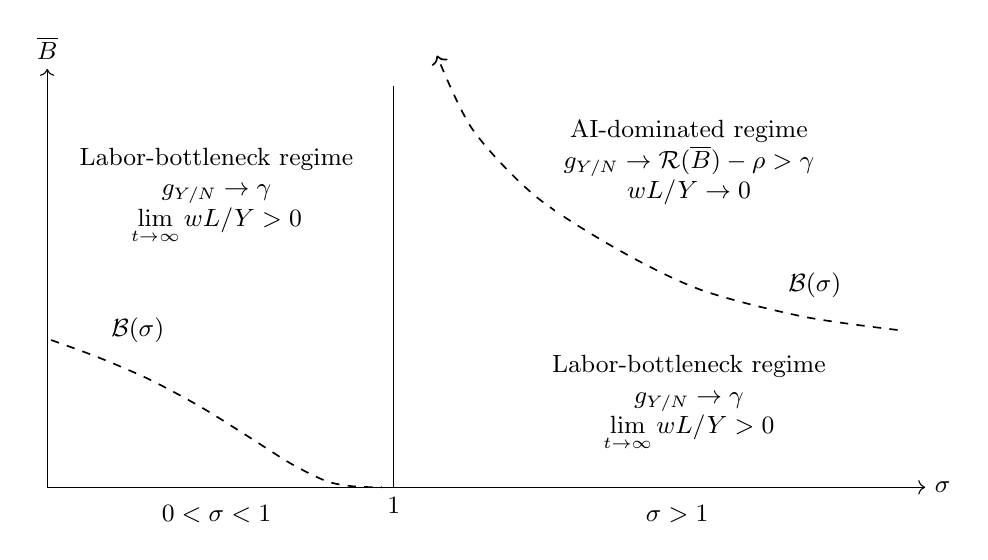
\begin{tikzpicture}[
 x=1.00cm,y=0.85cm,
 every node/.style={font=\small},
 regime/.style={align=center,inner sep=3pt,fill=white}
]
 \draw[->] (0,0) -- (11.15,0) node[right] {$\sigma$};
 \draw[->] (0,0) -- (0,6.25) node[above] {$\overline B$};
 \draw[semithick] (4.40,0) -- (4.40,6.00);
 \node[below] at (4.40,0) {$1$};
 \node[below] at (2.15,-0.12) {$0<\sigma<1$};
 \node[below] at (8.00,-0.12) {$\sigma>1$};

 % The complementary branch approaches zero as sigma approaches one
 % from below. It is not a continuation of the gross-substitutes branch.
 \draw[semithick,dashed]
  plot[smooth] coordinates
  {(0.05,2.20) (0.65,1.94) (1.30,1.61) (1.95,1.20)
   (2.55,0.76) (3.10,0.35) (3.55,0.09) (3.90,0.012)
   (4.25,0.001)};
 \node[regime] at (2.15,4.35)
  {Labor-bottleneck regime\\
   $g_{Y/N}\to\gamma$\\
   $\displaystyle\lim_{t\to\infty}wL/Y>0$};
 \node[regime] at (1.15,2.35) {$\mathcal B(\sigma)$};

 \draw[semithick,dashed,->]
  plot[smooth] coordinates
  {(10.80,2.35) (9.60,2.55) (8.30,2.95) (7.25,3.55)
   (6.20,4.35) (5.40,5.35) (4.95,6.45)};

 \node[regime] at (8.15,4.85)
  {AI-dominated regime\\
   $g_{Y/N}\to \mathcal R(\overline B)-\rho>\gamma$\\
   $wL/Y\to0$};
 \node[regime] at (8.15,1.25)
  {Labor-bottleneck regime\\
   $g_{Y/N}\to\gamma$\\
   $\displaystyle\lim_{t\to\infty}wL/Y>0$};
 \node[regime] at (9.75,3.02) {$\mathcal B(\sigma)$};
\end{tikzpicture}%
}
\caption{Constructed finite-frontier regimes. The vertical axis is linear
and the curves are schematic rather than calibrated. For $0<\sigma<1$,
$\overline B>\mathcal B(\sigma)$ is the condition for the positive-labor-share
construction in Proposition~\ref{prop:rewrite-capped-complements-existence}. For $\sigma>1$,
the curve separates the labor-bottleneck and AI-dominated equilibria in
Proposition~\ref{prop:rewrite-capped-substitutes-labor-existence}
and~\ref{prop:rewrite-capped-substitutes-existence}.}
\label{fig:rewrite-frontier-regimes}
\end{figure}


The identity $wL/Y=(1-\alpha)(1-s_X)$ translates these limits into income shares. Labor retains a positive share in the first three cases and a vanishing share in the fourth. At unit elasticity, its share is exactly $(1-\alpha)\omega_L$ at every date; correspondingly, $p_XX/Y=(1-\alpha)\omega_X$, whereas $s_X=\omega_X$. Write $\overline r=\lim_{t\to\infty}r_t$ along a constructed equilibrium. Table~\ref{tab:rewrite-finite-existence} summarizes the four cases.

\begin{table}[H]
\centering
\caption{Constructed finite-frontier equilibria}
\label{tab:rewrite-finite-existence}
\small
\begin{tabular}{@{}llll@{}}
\toprule
Elasticity & AI Efficiency & $\lim g_{Y/N}$ & $\lim wL/Y$ \\
\midrule
$0<\sigma<1$ & $\overline B>\mathcal B(\sigma)$ & $\gamma$ & Positive \\
$\sigma=1$ & Any finite $\overline B>0$ & $\gamma$ & $(1-\alpha)\omega_L$ \\
$\sigma>1$ & $\overline B<\mathcal B(\sigma)$ & $\gamma$ & Positive \\
$\sigma>1$ & $\overline B>\mathcal B(\sigma)$ & $\mathcal R(\overline B) -\rho>\gamma$ & Zero \\
\bottomrule
\end{tabular}
\end{table}

For $\sigma>1$, the strict inequalities distinguish the two equilibrium
families in Proposition~\ref{prop:rewrite-equilibrium-regimes}:
\begin{itemize}
 \item If $\mathcal R(\overline B)<\rho+\gamma$, equivalently
 $\overline B<\mathcal B(\sigma)$, the return at a vanishing labor share
 cannot sustain growth faster than effective labor. The constructed
 equilibrium retains a positive labor share, and its actual interest rate
 converges to $\rho+\gamma$, not to $\mathcal R(\overline B)$.
 \item If $\mathcal R(\overline B)>\rho+\gamma$, equivalently
 $\overline B>\mathcal B(\sigma)$, the return supports growth faster than
 effective labor even as labor's share vanishes. Along the constructed
 AI-dominated equilibrium, $r\to\mathcal R(\overline B)$ and output per
 person grows asymptotically at $\mathcal R(\overline B)-\rho>\gamma$.
 \item If $\mathcal R(\overline B)=\rho+\gamma$, the two return formulas
 coincide. This equality identifies the boundary between the strict
 regimes, but the existence proof does not cover it. It establishes
 neither existence nor nonexistence of an equilibrium at the threshold.
\end{itemize}
I use this comparison as an economic regime threshold only for $\sigma>1$.
For $\sigma<1$, $s_X\to1$ corresponds instead to AI services becoming scarce
relative to effective labor. The condition
$\overline B>\mathcal B(\sigma)$, or
$\mathcal R(\overline B)>\rho+\gamma$, is then only a sufficient condition
for the positive-labor-share construction in
Proposition~\ref{prop:rewrite-capped-complements-existence}; it does not
imply AI-dominated growth.

The proof first expresses growing quantities and shrinking efficiency gaps
in units with finite limits. For each parameter configuration covered by
the proposition, I conjecture a stationary point of these normalized
dynamics and derive its values from the model. I then construct
trajectories from every sufficiently nearby admissible initial state,
selecting $C_0,q_0$ and verifying agent optimality and both transversality
conditions. The initial stocks need not lie on a balanced-growth path.

This result is local in initial states, not in time. Closeness concerns
capital, the remaining AI-efficiency gap, and the scale of effective labor
jointly; $B_0$ close to $\overline B$ alone is not sufficient. The precise
sets and local uniqueness result are given in the proof. Existence from
arbitrary initial states and global uniqueness are not established.
These analytical limits also guide the algorithm's boundary conditions
(Appendix~\ref{app:rewrite-algorithm}), but do not determine the duration
or shape of the transition.

Across these equilibrium regimes, long-run real-wage growth exceeds $\gamma$ if and
only if labor's income share converges to zero.
Proposition~\ref{prop:rewrite-output-wage-wedge} in
Appendix~\ref{app:rewrite-proofs} derives the exact relationship between
the wage-growth premium and the decline in labor's income share.

\subsection{Raising the AI-efficiency frontier}
\label{subsec:rewrite-growth-frontier}

The constructed trajectories have convergent growth rates and a positive
limiting consumption--output ratio. Consumption and output therefore have
the same limiting growth rate. The household Euler equation gives
\begin{equation}
 \lim_{t\to\infty}\frac{\mathrm d\log(Y_t/N_t)}{\mathrm dt}
 =\lim_{t\to\infty}(g_C-n)=\overline r-\rho.
 \label{eq:rewrite-long-run-growth-return}
\end{equation}
These are limits of equilibrium transitions, not restrictions imposed on
their growth rates at every date.

\Needspace{4\baselineskip}
Holding $\sigma>1$ and all other parameters fixed, the constructed families
give the following comparative statics across finite frontiers:
\begin{equation}
 \overline r(\overline B;\sigma)=
 \begin{cases}
  \rho+\gamma,&\mathcal R(\overline B)<\rho+\gamma,\\[2pt]
  \mathcal R(\overline B),&\mathcal R(\overline B)>\rho+\gamma.
 \end{cases}
 \label{eq:rewrite-interest-frontier}
\end{equation}
Below the threshold, a larger frontier does not change the limiting
interest or growth rate. Above it,
\begin{equation}
 \frac{\partial\overline r}{\partial\overline B}
 =\frac{1-\alpha}{\alpha}
 \frac{\mathcal R(\overline B)+\delta}{\overline B}>0,
 \qquad
 \lim_{\overline B\to\infty}\overline r(\overline B;\sigma)=\infty.
 \label{eq:rewrite-interest-frontier-derivative}
\end{equation}
The limiting growth rate per person has the same derivative because it
equals $\overline r-\rho$. The two interest-rate formulas approach
$\rho+\gamma$ at the threshold, although the existence proof does not cover
equality. For $\sigma=1$, and for the constructed complementary-input
family, $\overline r=\rho+\gamma$ instead remains independent of the frontier.

\subsection{The uncapped economy and the role of the frontier}
\label{subsec:rewrite-uncapped}

The comparative static in
\eqref{eq:rewrite-interest-frontier-derivative} does not solve the economy
with an infinite AI-efficiency frontier. It first fixes a finite
$\overline B$, constructs an equilibrium, takes that
economy's long-run limit, and only then compares the resulting limits as
$\overline B$ increases. Setting $\overline B=\infty$ at the outset changes
the state equation by setting $\psi(B)=1$ and removes the bound on the
developer's state. In general,
\begin{equation}
 \lim_{\overline B\to\infty}\lim_{t\to\infty}r_t(\overline B)
 \quad\text{need not equal}\quad
 \lim_{t\to\infty}r_t(\infty),
 \label{eq:rewrite-noncommuting-limits}
\end{equation}
and the expression on the right may not exist. The initial-stock
neighborhood and the equilibrium choices of $C_0$ and $q_0$ also depend on
the frontier. Existence for every fixed finite frontier therefore does not
imply existence in the uncapped economy.

This distinction is especially important when $\sigma>1$. At high AI
efficiency, effective AI production services can replace labor. Holding
current $K,A,$ and $L$ fixed, optimized operating profit then grows
asymptotically in proportion to $KB^{(1-\alpha)/\alpha}$. Research raises
$B$, and a higher $B$ both raises operating profit and makes subsequent
research compute more productive. The capped equilibria reveal the strength
of this feedback: once the economy is in the AI-dominated regime, the
limiting interest and output-growth rates increase with $\overline B$ and
become unbounded as $\overline B\to\infty$. This divergence is evidence that
the uncapped problem may behave qualitatively differently. It is not, by
itself, proof of a finite-time singularity or of equilibrium nonexistence.
No analogous divergence appears in the finite-frontier equilibria constructed
for $\sigma\leq1$, where labor remains a long-run bottleneck. This does not
establish existence without a frontier in those cases either.

The developer's optimization problem identifies a more immediate possible
failure. Proposition~\ref{prop:rewrite-research-scale} in
Appendix~\ref{app:rewrite-proofs} shows that, in the uncapped economy,
the condition $\eta<\alpha$ makes the benefit generated by a
large research expenditure grow at most sublinearly in that expenditure on
a fixed finite horizon, while its cost grows linearly. It therefore rules out
an arbitrarily large research burst as the developer's optimal response in
that partial-equilibrium problem. If instead $\sigma>1$ and $\eta>\alpha$,
the developer can make its finite-horizon payoff arbitrarily large by
increasing an early research burst. No finite research plan maximizes its
objective. At $\eta=\alpha$, the outcome depends on the coefficients of the
leading benefit and cost terms. These results explain why $\eta<\alpha$ is a
substantive restriction, but they still do not establish an uncapped
infinite-horizon general equilibrium.

The failure when the developer's value is unbounded is economic rather than
numerical. Research compute $M$ is a use of the final good, not merely a
financial position. The household may finance a negative distribution from
the developer, but finance cannot create the real resources used in research.
Equation~\eqref{eq:rewrite-eq-kdot} requires research to compete with
consumption, inference compute, and physical investment. If every finite
research plan can be improved by choosing a larger research burst, no
allocation with finite resources can satisfy the developer's optimality
condition and the aggregate resource constraint at the same time. Such an
allocation is not an equilibrium under
Definition~\ref{def:rewrite-equilibrium}.

A different failure can occur even when the developer's value is bounded on
every finite horizon. Recursive improvement may cause $B$, output, capital,
or research expenditure to become unbounded at a finite date. I use
\emph{finite-time singularity} for this event, rather than for merely rapid
growth. A path that ends at such a date is not an equilibrium
as defined in Section~\ref{sec:rewrite-model}: it does not provide finite,
feasible allocations for every $t\geq0$, and its infinite-horizon optimality
and transversality conditions are not defined. The analysis in this paper
does not prove that every uncapped trajectory with $\sigma>1$ reaches such a
singularity. It also does not rule out an uncapped equilibrium that remains
finite at every finite date. Explosive-growth mechanisms in
\citet{nordhaus2021} and \citet{davidsonetal2026} motivate this question but
do not replace the missing equilibrium argument for the present model.

I therefore use a finite frontier as an analytical continuation device, not
as an estimate of a permanent technological ceiling. For each finite
$\overline B$, the term $1-B/\overline B$ keeps AI efficiency in a bounded
state space and makes it possible to establish and compute an equilibrium.
I then raise the frontier and examine how the equilibrium regime, growth,
interest rates, and income shares change. This strategy separates results
that hold for every fixed finite frontier from claims about an uncapped
economy. If the capped equilibria fail to converge, or their limiting growth
rates diverge, the correct conclusion is that this continuation does not
produce an uncapped equilibrium---not that a finite-time singularity has
already been proved.

\section{Quantitative equilibrium paths}
\label{sec:rewrite-quantitative}

\subsection{Parameters and initial conditions}
\label{subsec:rewrite-calibration}

I compare four economies with the same parameters and predetermined initial
stocks, varying only $\sigma$. Table~\ref{tab:rewrite-parameters} retains the
macroeconomic benchmarks used in the earlier specification. The AI parameters
are illustrative, not estimated. All four economies have autonomous research
and a positive AI weight; the no-AI economy in Remark~\ref{rem:rewrite-no-ai}
is not one of these four scenarios.

\begin{table}[H]
\centering
\caption{Parameters and scenario choices}
\label{tab:rewrite-parameters}
\small
\setlength{\tabcolsep}{4pt}
\renewcommand{\arraystretch}{1.10}
\begin{tabular}{P{0.10\textwidth}P{0.17\textwidth}P{0.27\textwidth}P{0.35\textwidth}}
\toprule
Parameter & Value & Interpretation & Source or rationale\\
\midrule
$\alpha$ & 0.33 & Capital elasticity & Standard one-third macro benchmark\\
$\delta$ & 0.05 & Annual capital depreciation & Annual benchmark; PWT comparison \citep{pwt110}\\
$\rho$ & 0.04 & Annual household discount rate & Preference calibration\\
$n$ & 0.003 & Annual population growth & Constant-rate approximation to the UN 2024--2100 world projection \citep{unwpp2024}\\
$\gamma$ & 0.01 & Annual growth of labor-augmenting technology & Illustrative long-run trend; see \citet{oecdlongrun2025}\\
$\omega_X$ & 0.20 & Weight on effective AI production services & Scenario choice, not an observed industry share\\
$\omega_L$ & 0.80 & Weight on effective labor & $1-\omega_X$\\
$\eta$ & 0.20 & Research exponent & Assumptions~\ref{ass:rewrite-research-curvature} and~\ref{ass:rewrite-research-concavity}\\
$\chi$ & 1.4378 & Research productivity & Calibrated transition-speed parameter\\
$\sigma$ & 0.90; 1; 1.10; 1.50 & AI--labor substitution & Four scenarios spanning the analytical regimes\\
$\overline B$ & $1.10\,\overline B_c(1.50)$ $\simeq170.124$ & Common AI-efficiency frontier & Ten percent above the threshold for $\sigma=1.50$\\
\bottomrule
\end{tabular}
\end{table}

The constant $n$ extrapolates a finite-period demographic approximation; it
is not a claim that the UN projects constant population growth forever.
The OECD benchmark for $\gamma$ concerns measured labor-productivity growth,
not $A$ directly. I use it only as an approximate guide to the magnitude of
long-run labor-augmenting technological progress.
The parameter $\chi$ determines research speed relative to the other annual
rates, so it is not merely a free time-unit normalization. I choose
$\chi=1.4378$ so that, in the $\sigma=1.50$ equilibrium, the labor income share
completes half of the distance between its date-zero value and its analytical
limit after 50 model years. This is an illustrative timing normalization, not
an estimate. Different values of $\chi$ produce faster or slower transitions
and require the entire equilibrium path to be solved again. The horizontal
axes below measure model years, not calendar forecasts. Likewise, the OECD's
discussion of AI-investment measurement supports treating $\omega_X$ as a
scenario parameter, but does not identify its value
\citep{oecdaiinvestment2025,oecdproductivity2026}.

The common frontier is below $\overline B_c(1.10)\simeq60.4$ million but above
$\overline B_c(1.50)\simeq154.658$. Thus $\sigma=1.10$ retains a positive
long-run labor share, whereas $\sigma=1.50$ enters the AI-dominated regime.
Changing the frontier separately across scenarios would confound this
comparison of elasticities.

I set
\begin{equation}
 A_0=N_0=1,\qquad K_0=4,\qquad B_0=0.10\overline B\simeq17.0124.
 \label{eq:rewrite-simulation-initial-stocks}
\end{equation}
These common initial stocks place the economy closer to the capped
$\sigma=1$ terminal regime than the earlier uncapped reference: initial AI
efficiency is 10 percent of its frontier and initial capital per unit of
effective labor is about 44 percent of its terminal $\sigma=1$ value. They are
not a balanced-growth state of the capped economy. An exact constant-efficiency reference at
$B_0=\overline B$ would eliminate further improvements in AI efficiency and would
lie outside the interior problem studied here. In each capped economy, the
BVP selects $C_0$ and $q_0$ anew; neither jump variable is fixed at its
uncapped reference value.

\subsection{Numerical method and equilibrium admission}
\label{subsec:rewrite-method}

I retain the four-dimensional boundary-value architecture: two initial stock
conditions and two terminal conditions selecting the stable equilibrium
continuation. The appropriate finite-frontier regime from
Section~\ref{sec:rewrite-regimes}, not the uncapped unit-elastic BGP, determines
the terminal conditions. Appendix~\ref{app:rewrite-algorithm} documents the
continuation, equation reconstruction, and numerical checks.

In economic terms, the algorithm takes $K_0$ and $B_0$ as given and selects
the initial consumption and shadow value that place the economy on the stable
equilibrium path. It first constructs that path near the analytically
characterized terminal regime and then moves it gradually to the prescribed
initial stocks. Solving the boundary-value problem is only the construction
step; the separate admission tests determine whether the resulting candidate
is reported as an equilibrium.

A converged BVP is not sufficient for admission. I also check feasibility,
independently reconstructed dynamic residuals, stability to longer horizons
and tighter tolerances, both transversality conditions, and sufficient global
developer optimality. The first three scenarios satisfy the global concavity
test. For $\sigma=1.50$, that stronger test fails at low counterfactual
AI-efficiency levels, but the Hamiltonian support test in
Proposition~\ref{prop:rewrite-hamiltonian-support} passes. Its analytical
long-run bound is given in \eqref{eq:rewrite-support-terminal-bound}.

\subsection{Growth, prices, and the distribution of output}
\label{subsec:rewrite-distribution}

Figures~\ref{fig:rewrite-accumulation-growth}--\ref{fig:rewrite-ai-distribution}
present the transition in three steps: quantities and accumulation, prices and
returns, and the distribution of output. Each panel includes the same four
admitted trajectories. The three labor-bottleneck paths consequently appear
close to one another in several panels. This compression reflects their common
long-run regime; exact initial and limiting values of the central outcomes are
reported in Table~\ref{tab:rewrite-central-path-values}.

\Needspace{10\baselineskip}
The relative growth of effective AI production services is central to reading
the figures. Rearranging \eqref{eq:rewrite-sx} gives
\begin{equation}
 \frac{s_X}{1-s_X}
 =\frac{\omega_X}{\omega_L}
 \left(\frac{X}{AL}\right)^{(\sigma-1)/\sigma}.
 \label{eq:rewrite-transition-share-odds}
\end{equation}
Differentiating this expression yields
\begin{equation}
 \frac{d}{dt}\log\!\left(\frac{s_X}{1-s_X}\right)
 =\frac{\sigma-1}{\sigma}\left[g_X-(n+\gamma)\right].
 \label{eq:rewrite-transition-share-growth}
\end{equation}
Thus the growth of $X/(AL)$ determines the direction and speed at which the
AI share changes, conditional on $\sigma$.

Figure~\ref{fig:rewrite-accumulation-growth} first reports the growth rates of
output, effective AI production services, and capital per unit of effective
labor. These are $g_Y-(n+\gamma)$, $g_X-(n+\gamma)$, and
$g_K-(n+\gamma)$, respectively. Growth rates show when the economy accelerates
without compressing the large level differences that emerge across regimes.

\begin{figure}[H]
 \centering
 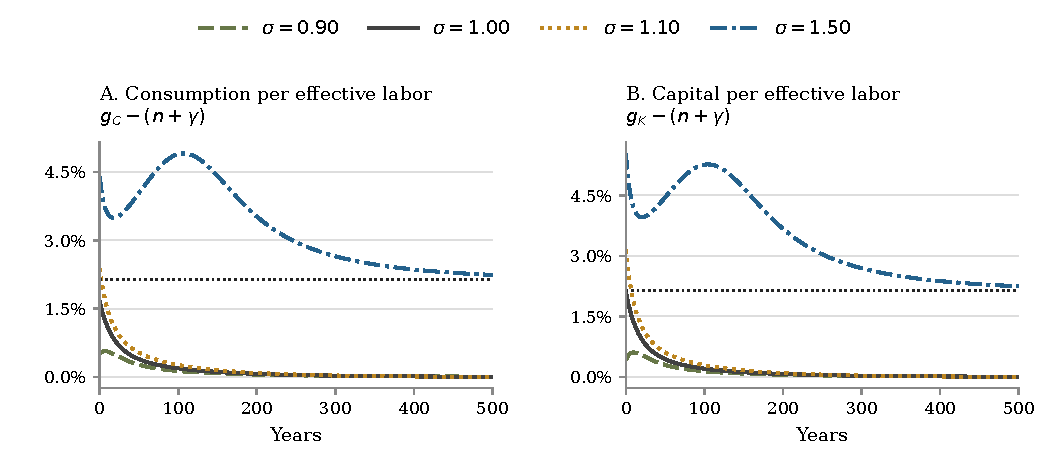
\includegraphics[width=\textwidth]{figures_rewrite/equilibrium_accumulation_growth.pdf}
 \caption{Growth of output, effective AI production services, and capital per
 unit of effective labor. Each panel compares the same four admitted numerical
 equilibrium trajectories over 500 model years. Panels A and C use the same
 linear percentage scale; Panel B uses a separate linear percentage range.
 Thin horizontal dotted lines mark the analytical limits for $\sigma=1.50$.}
 \label{fig:rewrite-accumulation-growth}
\end{figure}

\Needspace{10\baselineskip}
Figure~\ref{fig:rewrite-growth-returns} next reports real-wage growth, the net
interest rate, and the price of effective AI production services. The first
two are rates; $p_X$ is a relative-price level measured in units of the final
good. Equation~\eqref{eq:rewrite-markup} implies
$p_X=1/[B(1-e_X)]$. Because $B$ approaches its finite frontier and $e_X$
approaches a value below one in every terminal regime, $p_X$ converges to a
positive finite level. It falls rather than grows without bound in all four
simulations. I therefore report its level on a logarithmic scale, which keeps
the four positive price paths visible despite their different magnitudes.

\begin{figure}[H]
 \centering
 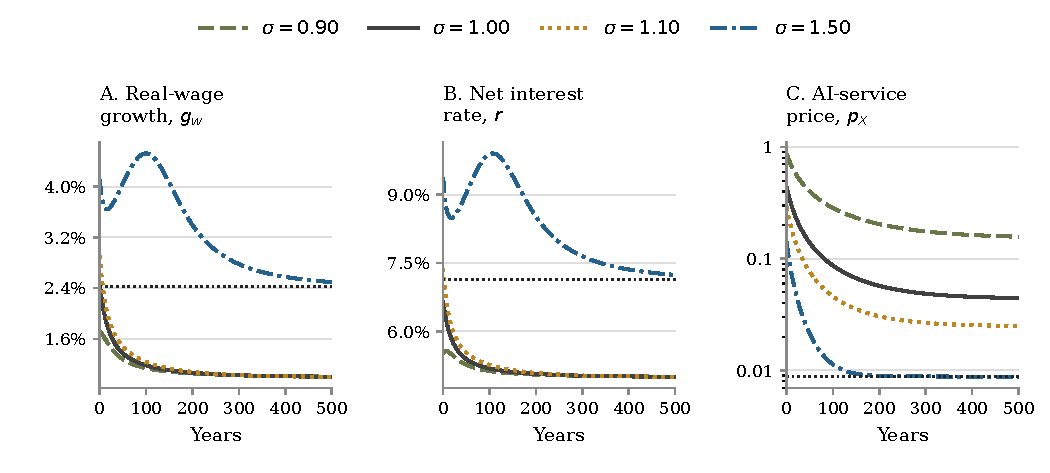
\includegraphics[width=\textwidth]{figures_rewrite/equilibrium_growth_returns.pdf}
 \caption{Wages, returns, and the AI-service price. Each panel compares the same
 four admitted numerical equilibrium trajectories over 500 model years.
 Real-wage growth and the net interest rate use linear percentage scales.
 The level of $p_X$ uses a logarithmic scale. Thin horizontal dotted lines mark
 the analytical limits for $\sigma=1.50$.}
 \label{fig:rewrite-growth-returns}
\end{figure}

Finally, Figure~\ref{fig:rewrite-ai-distribution} reports labor income and the
three uses of AI-industry revenue as shares of final output. Combining final-good
zero profit with $\Pi=p_XX-U-M$ gives
\begin{equation}
 \frac{wL}{Y}+\frac{\Pi}{Y}+\frac{U}{Y}+\frac{M}{Y}=1-\alpha.
 \label{eq:rewrite-noncapital-distribution}
\end{equation}
The four panels therefore exhaust the noncapital share of output. Gross capital
income, $(r+\delta)K/Y=\alpha$, is constant and accounts for the remainder.

\begin{figure}[H]
 \centering
 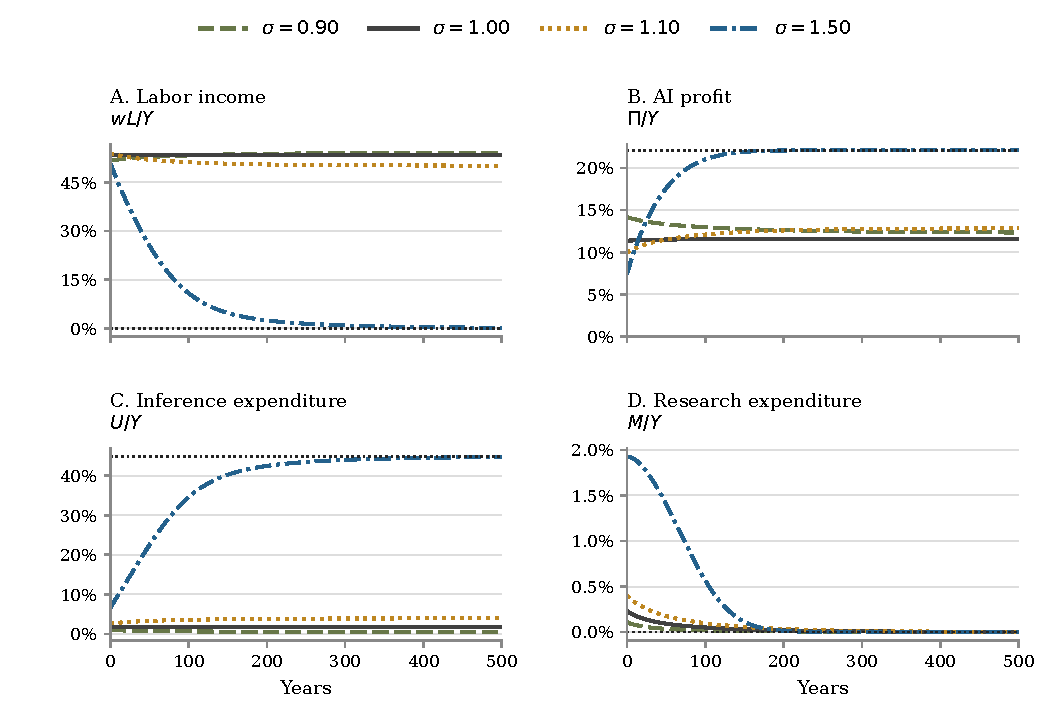
\includegraphics[width=\textwidth]{figures_rewrite/equilibrium_ai_distribution.pdf}
 \caption{Distribution of the noncapital share of output. The panels report
 labor income, AI profit, inference expenditure, and research expenditure,
 each divided by final output. Together they sum to $1-\alpha$; the omitted
 gross capital-income share is the constant $\alpha$. Each panel compares the
 same four admitted numerical equilibrium trajectories over 500 model years
 and uses a linear percentage scale. Thin horizontal dotted lines mark the
 analytical limits for $\sigma=1.50$.}
 \label{fig:rewrite-ai-distribution}
\end{figure}

\begin{table}[H]
\centering
\caption{Initial and long-run values of the central outcomes}
\label{tab:rewrite-central-path-values}
\small
\setlength{\tabcolsep}{5pt}
\begin{tabular}{ccrrrrr}
\toprule
$\sigma$ & Date & $g_Y-n$ & $g_w$ & $r$ & $wL/Y$ & $p_XX/Y$\\
\midrule
0.90 & $0$      & 1.629 & 1.711 & 5.508 & 51.7 & 15.3\\
     & $\infty$ & 1.000 & 1.000 & 5.000 & 54.2 & 12.8\\
1.00 & $0$      & 2.458 & 2.458 & 6.646 & 53.6 & 13.4\\
     & $\infty$ & 1.000 & 1.000 & 5.000 & 53.6 & 13.4\\
1.10 & $0$      & 3.046 & 2.909 & 7.380 & 54.0 & 13.0\\
     & $\infty$ & 1.000 & 1.000 & 5.000 & 50.2 & 16.8\\
1.50 & $0$      & 5.390 & 4.115 & 9.385 & 51.0 & 16.0\\
     & $\infty$ & 3.135 & 2.423 & 7.135 & 0.0 & 67.0\\
\bottomrule
\end{tabular}

\vspace{2pt}
\parbox{0.94\textwidth}{\footnotesize\emph{Note:} All entries are percentages.
Date-zero entries come from the numerical equilibrium paths. Infinite-date
entries are the analytical limits characterized in Section~\ref{sec:rewrite-regimes}.}
\end{table}

The first three scenarios approach per-person growth of $1\%$ and a net
interest rate of $5\%$. For $\sigma=1.50$, their analytical limits are
$3.135\%$ and $7.135\%$, respectively. Real wages then grow asymptotically
at $2.423\%$. Thus output per person grows $0.712$ percentage points faster
than the real wage. By Proposition~\ref{prop:rewrite-output-wage-wedge}, this
implies an asymptotic decline of $0.712\%$ per year in the log labor income
share. The central distributional result is therefore not that real wages decline:
workers become richer in absolute terms while their claim on total output
vanishes. AI revenue meanwhile approaches $67\%$ of output. These limiting
rates describe the equilibrium continuations; they are not imposed as
constant rates during the transition.

The AI-dominated path also displays signals before labor's income share has
fallen sharply. At date zero, $X/(AL)$ grows at $16.051\%$ and the net interest
rate is $9.385\%$, well above the $5\%$ labor-bottleneck benchmark, while labor
still receives $51.0\%$ of output. Moreover, because $L=N$, the accounting
identity
\begin{equation}
 \frac{d}{dt}\log\!\left(\frac{wL}{Y}\right)
 =g_w-(g_Y-n)
 \label{eq:rewrite-transition-labor-share-identity}
\end{equation}
holds at every date. The gap between output-per-person and real-wage growth
therefore does not merely predict a later distributional change: a positive
gap is exactly the contemporaneous rate at which the log labor income share
declines, and a widening gap means that decline is accelerating.

Equations~\eqref{eq:rewrite-transition-share-odds} and
\eqref{eq:rewrite-transition-share-growth} provide the structural explanation
for the speed of the transition. A value $\sigma>1$ makes the AI share rise
with $X/(AL)$, but it does not make
AI immediately replace labor. When $\sigma$ is close to one, the exponent
$(\sigma-1)/\sigma$ is small and the share responds slowly even to large
increases in relative AI services. At $\sigma=1.50$, for example, the
exponent is $1/3$: increasing the odds $s_X/(1-s_X)$ by a factor of ten
requires a thousand-fold increase in $X/(AL)$. For elasticities closer to
one, the required increase is larger still, conditional on the frontier
being high enough to support the AI-dominated regime.

The economy must also accumulate the inputs that produce this change.
Neither $K$ nor $B$ can jump. Expanding $X$ requires inference compute
$U=X/B$, while improving $B$ requires research compute $M$; both uses compete
with consumption and physical investment for current output. Moreover,
$\eta=0.20$ implies strong diminishing returns to a contemporaneous increase
in research compute. As $B$ rises, however, it reduces the compute required
to supply a unit of $X$ and makes subsequent research compute more productive.
The feedback therefore strengthens gradually. Near the finite frontier,
$\psi(B)$ slows further efficiency improvement. The eventual acceleration in
the AI-dominated equilibrium is consequently not an explosion of $B$: it is
sustained by the expansion of capital and effective AI production services
after labor ceases to be the binding input.

The date of takeoff is not a structural prediction of the model. Equation
\eqref{eq:rewrite-transition-share-odds} implies an earlier transition when
$\sigma$ is farther above one or when $X$ grows faster relative to $AL$.
Within the model, greater research productivity $\chi$, a higher initial
$B_0$, or a larger AI weight $\omega_X$ can advance the transition through
different channels. Faster capital accumulation or slower growth of effective
labor can also allow $X/(AL)$ to rise sooner. These changes are not
interchangeable: $\sigma$ and $\omega_X$ alter the production technology,
$B_0$ changes the initial economy, and $\chi$ changes the research clock. The
effects of changing $\eta$ or $\overline B$ on the takeoff date do not have an
unambiguous general-equilibrium sign because they also change research
incentives and the terminal equilibrium. These comparative mechanisms indicate
how the transition may move, but do not identify a date without recalculating
the equilibrium path.

The $\sigma=1.50$ path displays this mechanism under the calibrated research
speed. The labor share completes 10 percent of its decline after 8.3 model
years, half after 50 years, and 90 percent after 145.2 years. At year 50,
output per person grows at $5.616\%$, the real wage at $4.050\%$, and labor
receives $25.5\%$ of output. At year 100, the corresponding growth rates are
$6.290\%$ and $4.522\%$, while labor's share has fallen to $10.9\%$. By year
500, output-per-person growth is $3.239\%$, real-wage growth is $2.494\%$,
and labor's share is $0.19\%$; all three are close to their analytical limits.
The non-monotone growth response reflects the costly initial research surge,
the subsequent acceleration in effective AI services, and eventual convergence
as $B$ approaches its frontier. These dates illustrate an equilibrium under
one research-speed calibration. They are not estimates of when an actual AI
transition will occur.

Substitution alone does not produce this outcome. With the same frontier
and $\sigma=1.10$, the labor share instead approaches $50.2\%$, compared
with $53.6\%$ at $\sigma=1$ and $54.2\%$ at $\sigma=0.90$.
The frontier's position relative to the elasticity-specific threshold is
essential to interpreting the comparison.

\subsection{Near-terminal labor-bottleneck paths}
\label{subsec:rewrite-near-terminal}

The initially high and declining growth rates of the three labor-bottleneck
paths in the main comparison are not their long-run prediction. They partly
reflect the distance between the common initial stocks in
\eqref{eq:rewrite-simulation-initial-stocks} and each economy's terminal
allocation. To isolate terminal behavior, I solve an additional exercise only
for $\sigma\in\{0.90,1,1.10\}$. I set
\begin{equation}
 \frac{B_0}{\overline B}=0.99,
 \qquad
 \frac{K_0}{A_0N_0}=
 \left.\frac{K}{AN}\right|_{\text{terminal}}
 =\begin{cases}
  6.5571,&\sigma=0.90,\\
  9.0990,&\sigma=1,\\
  12.2652,&\sigma=1.10.
 \end{cases}
 \label{eq:rewrite-near-terminal-stocks}
\end{equation}
Consumption and the developer's shadow value are again selected by the BVP
for each path. Because $B_0<\overline B$ and research remains positive, these
are not exact steady states at a finite date. They are equilibrium paths that
begin near their respective terminal regimes. Moreover, because the initial
capital ratio varies with $\sigma$, this exercise isolates terminal behavior;
it is not a comparative experiment holding all initial stocks fixed.

\begin{figure}[H]
 \centering
 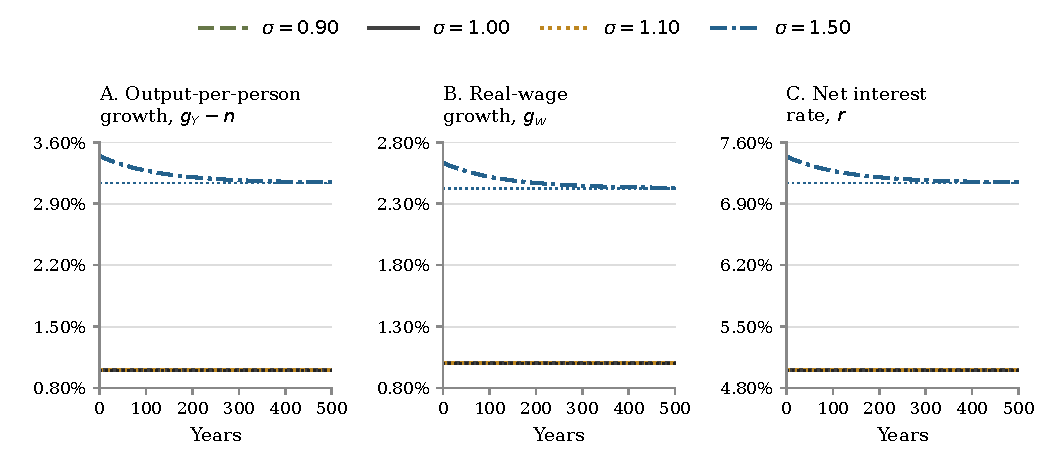
\includegraphics[width=\textwidth]{figures_rewrite/equilibrium_near_terminal_growth_returns.pdf}
 \caption{Near-terminal labor-bottleneck equilibrium paths. The panels report
 output-per-person growth, real-wage growth, and the net interest rate for
 three independently admitted numerical equilibria over 500 model years.
 Thin horizontal dotted lines mark their common analytical limits: $\gamma$
 for both growth rates and $\rho+\gamma$ for the net interest rate. The
 vertical axes cover narrow ranges around those limits.}
 \label{fig:rewrite-near-terminal-growth-returns}
\end{figure}

Figure~\ref{fig:rewrite-near-terminal-growth-returns} removes the large
date-zero movements visible in the main comparison. At date zero,
output-per-person and real-wage growth lie between $0.986\%$ and $0.994\%$,
while the net interest rate lies between $4.977\%$ and $4.990\%$. The three
paths then remain close to, and converge toward, their common analytical
limits of $1\%$, $1\%$, and $5\%$. The exercise therefore confirms that the
high initial growth rates in the main labor-bottleneck paths are transitional
responses to the common starting stocks, rather than properties of the
labor-bottleneck long run.

\subsection{A slower transition}
\label{subsec:rewrite-slow-transition}

The 50-year midpoint in the main comparison is a timing calibration rather
than a prediction. To show how strongly the transition can stretch out, I
recover the earlier calibration with
\begin{equation}
 \chi=0.01,\qquad K_0=2.027733654,\qquad B_0=0.443670932.
 \label{eq:rewrite-slow-transition-design}
\end{equation}
All other parameters, the common frontier, and the four values of $\sigma$
are unchanged. These initial stocks come from the uncapped unit-elastic BGP,
but neither the initial consumption nor the initial shadow value is imported
from it. Both jump variables are solved again for each capped economy. The
exercise changes both research productivity and the initial distance from the
frontier, so it should not be interpreted as a one-parameter estimate of the
effect of $\chi$. Each of the four paths is independently re-solved and passes
the same equilibrium-admission tests as the main comparison.

Figures~\ref{fig:rewrite-slow-accumulation-growth}--
\ref{fig:rewrite-slow-ai-distribution} retain the variables, normalizations,
scenario order, and scale conventions of the main figures. The only
presentational change is the 4,000-year window needed to display the slower
adjustment.

\begin{figure}[H]
 \centering
 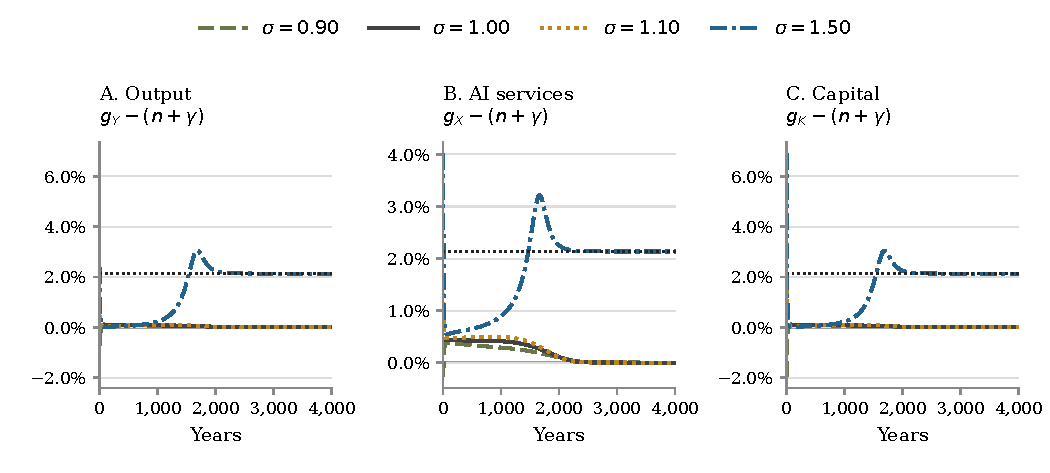
\includegraphics[width=\textwidth]{figures_rewrite/equilibrium_slow_accumulation_growth.pdf}
 \caption{Growth of output, effective AI production services, and capital per
 unit of effective labor under the slower-transition calibration. Each panel
 compares the same four admitted numerical equilibrium trajectories over
 4,000 model years. Panels A and C use the same linear percentage scale;
 Panel B uses a separate linear percentage range. Thin horizontal dotted
 lines mark the analytical limits for $\sigma=1.50$.}
 \label{fig:rewrite-slow-accumulation-growth}
\end{figure}

\begin{figure}[H]
 \centering
 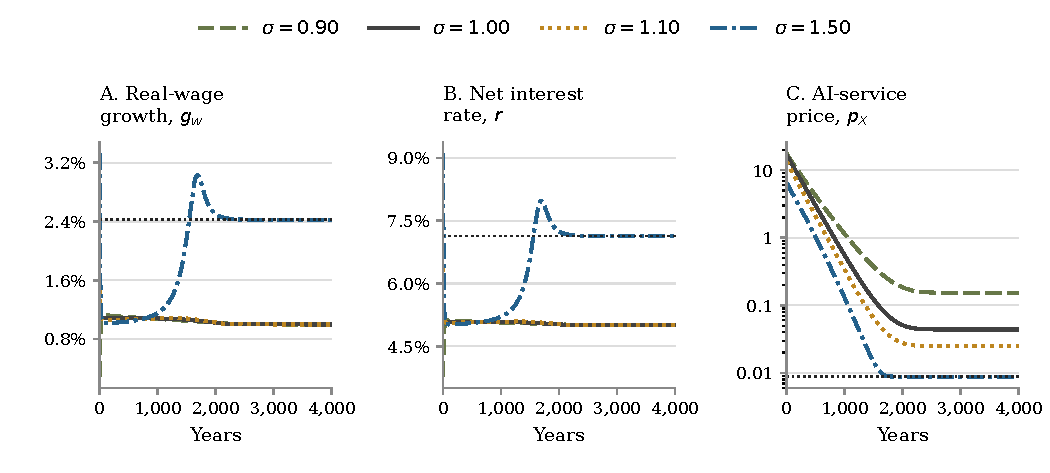
\includegraphics[width=\textwidth]{figures_rewrite/equilibrium_slow_growth_returns.pdf}
 \caption{Wages, returns, and the AI-service price under the slower-transition
 calibration. Each panel compares the same four admitted numerical equilibrium
 trajectories over 4,000 model years. Real-wage growth and the net interest
 rate use linear percentage scales; the level of $p_X$ uses a logarithmic
 scale. Thin horizontal dotted lines mark the analytical limits for
 $\sigma=1.50$.}
 \label{fig:rewrite-slow-growth-returns}
\end{figure}

\begin{figure}[H]
 \centering
 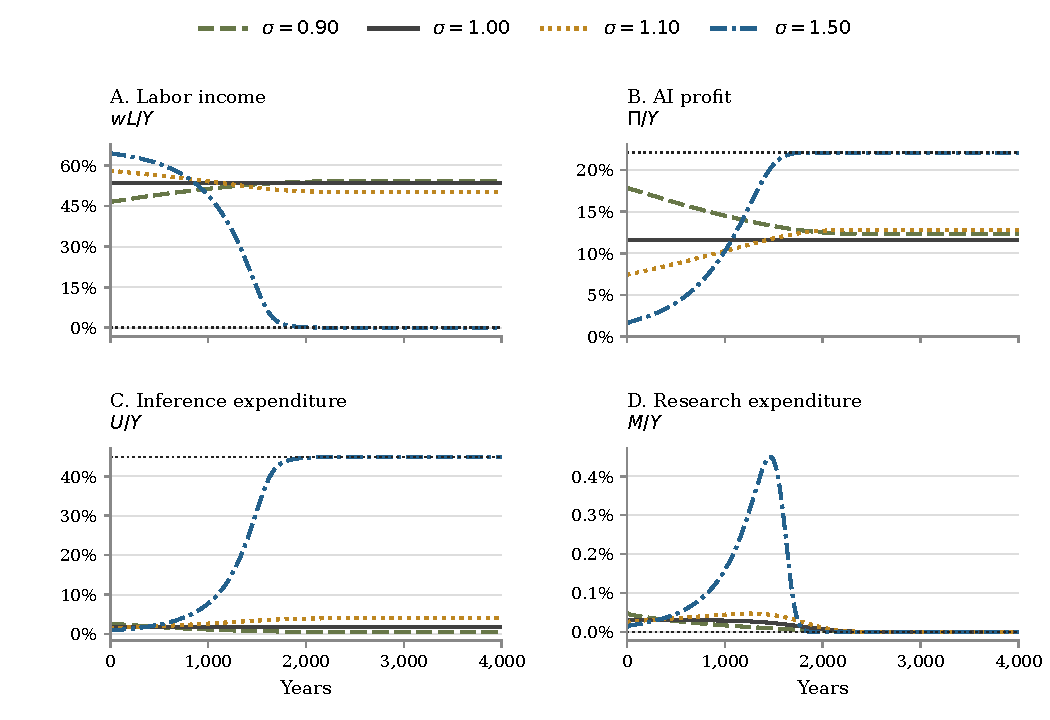
\includegraphics[width=\textwidth]{figures_rewrite/equilibrium_slow_ai_distribution.pdf}
 \caption{Distribution of the noncapital share of output under the
 slower-transition calibration. Labor income, AI profit, inference expenditure,
 and research expenditure are divided by final output and sum to $1-\alpha$.
 The omitted gross capital-income share is the constant $\alpha$. Each panel
 compares the same four admitted numerical equilibrium trajectories over
 4,000 model years. Thin horizontal dotted lines mark the analytical limits
 for $\sigma=1.50$.}
 \label{fig:rewrite-slow-ai-distribution}
\end{figure}

In the slow $\sigma=1.50$ equilibrium, labor's income share completes only
10 percent of its decline after 657 model years, half after 1,295 years, and
90 percent after 1,605 years. At year 500, output per person grows at
$1.062\%$, the real wage at $1.043\%$, and labor still receives $60.5\%$ of
output. By year 1,500, output-per-person growth has risen to $2.797\%$, while
labor's share has fallen to $14.5\%$. The analytical limits are the same as in
the main comparison because $\sigma$ and $\overline B$ are unchanged; what
changes radically is when the economy approaches them. The model can therefore
generate a long interval in which little appears to happen before growth and
the distribution of output change sharply. It does not identify which of the
two timing calibrations is empirically more plausible.

\subsection{Initial financing sensitivity}
\label{subsec:rewrite-technology-revenue}

Moving the common initial stocks closer to the $\sigma=1$ terminal regime
materially reduces the initial financing requirement. In the reported
$\sigma=1.50$ path, research absorbs $12.0\%$ of AI revenue, inference absorbs
$41.4\%$, and the developer distributes the remaining $46.6\%$ as profit.
These quantities equal $1.92\%$, $6.60\%$, and $7.44\%$ of final output,
respectively.

This benign date-zero composition is not invariant to the initial stocks. In
an admitted sensitivity path that begins much farther from the terminal regime,
at $K_0=2.0277$ and $B_0/\overline B=0.26\%$, and recalibrates $\chi$ to preserve
the same 50-year midpoint, research expenditure initially equals $106.0\%$ of
AI revenue and profit is $-40.5\%$ of AI revenue. The household owner then
finances the loss through an equity injection because current research raises
$B$ and the present value of future monopoly rents. The benchmark permits this intertemporal
financing: it imposes neither a borrowing constraint nor a nonnegative-profit
constraint on the developer. Adding such a constraint could delay or restrict
the transition. The contrast therefore identifies initial technological
distance and financing capacity as substantive determinants of the transition,
not as innocuous plotting choices.

In the AI-dominated limit, inference absorbs $67\%$ of AI revenue, research's
revenue share vanishes, and the developer retains $33\%$. Its net distribution
therefore approaches $22.11\%$ of final output. By contrast, at $\sigma=1$
AI revenue is always $13.4\%$ of output and inference absorbs $13.4\%$ of
that revenue. A vanishing research share does not mean that research stops:
the constructed finite-frontier equilibria have a positive limiting level of
research compute, while industry revenue continues to grow.

\section{Conclusion}
\label{sec:rewrite-conclusion}

The endogenous-growth model shows when improvements in AI efficiency generate
a temporary increase in growth and when they support a permanently
faster-growing economy. In the labor-bottleneck regime, the disappearance of
the growth premium does not imply that earlier gains in output and wages
disappear. In the AI-dominated regime, real wages grow permanently faster,
but output per worker grows faster still. Workers become better paid while
receiving a declining share of aggregate income.

These conclusions are conditional on the production and research technologies.
The link between permanently faster wage growth and a vanishing labor share
applies to the long-run regimes I characterize with a finite upper bound on
AI efficiency. Without this bound, the unit-elastic benchmark can instead
sustain faster growth with a positive labor share. The benchmark also assumes
autonomous AI research. Introducing human research tasks and allowing the
attainable level of efficiency to evolve would test how these assumptions
shape the results. The research networks and bottlenecks in
\citet{davidsonetal2026} offer a starting point, but their conditions for
explosive growth do not establish equilibrium existence in this model.

\ifshowlegacysimulations
The transition can be as important as the long-run outcome. In the calibrated
AI-dominated path, labor completes half of its income-share decline after 50
model years while output and wages grow rapidly. This timing is illustrative:
research productivity is not estimated, and changing it produces faster or
slower equilibrium adjustments rather than merely relabeling time. The initial
technological distance matters as well. The simulations nevertheless reveal
signals before most of the decline in labor's income share occurs: effective AI
production services can grow rapidly, the interest rate can rise above the
labor-bottleneck benchmark, and a positive output--wage growth gap shows that
labor's income share is already falling. Starting farther from the terminal
regime can require the developer's owner to finance large temporary losses
against future monopoly rents.
\else
The numerical exercises are illustrative rather than joint empirical fits to
AI revenues, research expenditure, and price changes. Research productivity
is particularly uncertain, so I place more weight on the conditional
long-run results than on the dates of takeoff. The measurement difficulties
documented by \citet{korinekmckelvey2026}, including limited information on
the allocation of compute, also constrain calibration. Moreover, the
experiments assume an unanticipated activation of RSI and omit adjustment
costs. An explicit compute sector with investment frictions, as in the GATE
model of \citet{erdiletal2025gate}, would allow me to examine whether the
large initial reallocations survive constraints on expanding compute capacity.
\fi

Permanent monopoly also restricts the interpretation of prices and profits.
Together with the production technology, it can imply a substantial AI revenue
share under complementarity even when the AI production weight is small.
I therefore retain this weight as an illustrative parameter rather than an
estimate of the industry's current size. \citet{korinekvipra2025} discuss
both forces toward concentration and competition among AI developers;
their analysis does not imply permanent monopoly. Allowing entry and
competition would make it possible to study how lower markups and the
prospect of losing market leadership affect private RSI investment.
AI revenue would still need to be distinguished from net profit after
inference and research costs.

The aggregate labor input also excludes differences across occupations and
the creation of new tasks in which workers retain a comparative advantage.
A task-based extension could incorporate the displacement and reinstatement
mechanisms of \citet{acemoglurestrepo2019}, allowing labor's role to change
through the creation and automation of tasks as well as through changes in
relative input use.
The present model cannot determine which workers gain or lose during
the transition.

Finally, a declining labor share does not by itself determine household
inequality or workers' economic power. The representative household owns
capital and the AI developer, so I do not distinguish workers who rely on
wages from households that receive most of the profits. As
\citet{jones2026future} emphasizes, asset ownership and redistribution matter
for who shares in AI-driven prosperity. Heterogeneous ownership and a fiscal
sector would allow me to study how capital income and transfers modify
the distribution of gains described here through wages and factor shares.

\enlargethispage{\baselineskip}
The central question is whether human labor remains sufficiently essential for
wages to keep pace with the economy as a whole.


\appendix
\section{Proofs}
\label{app:rewrite-proofs}

% Follow the order of propositions in the main text. Each proof must use only
% definitions and results that precede the proposition in the paper.

\clearpage
\section{Numerical algorithm and equilibrium audit}
\label{app:rewrite-algorithm}

% 1. Regime-specific normalization.
% 2. Boundary conditions and jump-variable selection.
% 3. Continuation in initial states, sigma_XL, and the finite frontier.
% 4. Exact reconstruction of equilibrium equations.
% 5. Horizon stability and both transversality conditions.
% 6. Developer optimality and the equilibrium-admission decision.
% 7. Reproducible file and code map.

\clearpage
\section{Conditional and excluded limits}
\label{app:rewrite-conditional-limits}

% Record useful conditional singular scalings and necessary restrictions on
% irregular continuations. Keep them separate from established equilibrium
% trajectories and state exactly which existence or optimality step is missing.


\bibliographystyle{apalike}
\bibliography{references}

\end{document}
